\chapter{Investigación y Desarrollo}

\section{Frameworks}

\subsection{No funcionales}

Para la implementaci\'on de nuestro sistema, originalmente, evaluamos la
utilizaci\'on de distintos frameworks disponibles. DeepQA, el producto
de IBM, no es de c\'odigo abierto, por lo que acerca de su
implementaci\'on s\'olo sabemos lo que ventilaron en sus art\'iculos
t\'ecnicos. Just.ask, el sistema basado en web comparado contra
OpenEphyra no est\'a disponible en la web al momento de escribir este
trabajo, mientras que OpenEphyra no funciona tal cual est\'a dise\~nado
originalmente (basado en web), sino que el autor sugiere unos pasos
esot\'ericos para configurarlo para usar conocimiento local. Cabe
destacar que esta falla en la funcionalidad est\'a asociada a la que
hab\'ia encontrado [AUTOR DE PAPER EPHYRA1] en Aranea y est\'a
vinculado con una serie de medidas restrictivas tomadas por las
compa\~n\'ias de buscadores, que fueron cerrando sus accesos gratuitos
para la comunidad de investigaci\'on bloqueando sus APIs y el acceso
autom\'atico a sus UI. Las alternativas para el uso de buscadores,
actualmente, se reducen a la configuraci\'on de una serie de proxies
sobre los que rotar el acceso a la UI y as\'i enga\~nar al detector de
accesos autom\'aticos -alternativa de legalidad cuestionable - o bien al 
pago por una quota de queries por mes.
OpenEphyra sobrevivi\'o a Aranea porque sus responsables escribieron
una interfaz para Bing cuando Google cerr\'o sus puertas, mientras que
los responsables de Aranea no lo hicieron. Finalmente, Bing tambi\'en
bloqueo el acceso autom\'atico gratuito. Notar que el mismo tipo de
discontinuaci\'on ocurri\'o con el API de traducciones de Google. La
empresa declara, expl\'icitamente, que no est\'a dispuesta a acceder a
ninguna quota de acceso gratuito para la investigaci\'on acad\'emica y
que todos sus servicios son pagos. 

%Tanto de Aranea como de OpenEphyra podr\'iamos llegar a tomar algunos de
%sus componentes a la hora de construir nuestro sistema. Por el momento,
%fueron simplemente dejados de lado.

\bigskip

\subsection{Qanus}

Finalmente, un sistema que \textit{s\'i} estaba disponible y funcionando
fue Qanus, que respetaba al pie de la letra su detalle t\'ecnico. Al comienzo
del proyecto, cont\'abamos con un corpus de datos en XML,
lo cual coincid\'ia, al menos en gran parte, con el input esperado de
la implementaci\'on Qa-sys. A pesar de esto, la adaptaci\'on de los
componentes no fue nada trivial y requiri\'o un tiempo excesivo. En
particular, exist\'ian dos opciones a la hora de construir un sistema
sobre la arquitectura Qanus: dejar de lado la implementaci\'on Qa-sys e
implementar todos los componentes de cero sobre la arquitectura, respetando las interfaces
dadas por el framework, o adaptar el sistema funcionando para que
trabaje sobre los nuevos datos y el nuevo entorno esperado. Frente a
esta alternativa, se aparece claro que el framework en s\'i mismo no
aporta demasiado, pues lo \'unico que hace es atar la implementaci\'on
final a una interfaz estructurada de tres procesos bastante sencillo.
Adem\'as, existe un cierto grado de dependencia de la arquitectura
hacia la implementaci\'on final, quiz\'as no a nivel t\'ecnico, pero si
en el modo en el que est\'a definida la estructura. Por este motivo,
encaramos una adaptaci\'on de Qa-sys a nuestro modelo de datos y a
nuestros requerimientos, pero los resultados no fueron buenos en
t\'erminos de resultados por tiempo invertido. El tiempo de aprendizaje
del framework mismo y el tiempo requerido para adaptar las distintas
componentes propias a las interfaces esperadas por Qanus es demasiado
alto para la soluci\'on que brinda. Como reci\'en mencionamos, en
realidad, el proceso de pipeline de tres pasos no tiene tantas aristas,
y adaptarse a un framework es mucho menos ameno que escribirlo. Este
puede ser uno de los motivos por los cuales, como acertadamente
se\~nalan los autores de Qanus, no existe ning\'un framework
estandarizado dentro del \'ambito de la investigaci\'on en QA.
Despu\'es de la investigaci\'on inicial, podr\'iamos concluir que
est\'a estandarizado, al menos a modo conceptual, la idea de que la
resoluci\'on del problema se debe enfocar como un pipeline de al menos
tres pasos que incluyen:
\begin{itemize}
\item el preprocesamiento de la base de conocimiento,
\item el preprocesamiento de la pregunta,
\item el retorno de la respuesta a partir de los resultados de los dos pasos anteriores. 
\end{itemize}
Como \'ultimo comentario al respecto, el modelo de Qanus resultaba poco atractivo
 a la hora de incorporar procesamiento en varios idiomas: el mejor approach
utilizando esta arquitectura era implementar dos sistemas basados en
Qanus paralelos y utilizar uno u otro de acuerdo con el resultado de
una detecci\'on inicial. 

\bigskip

Si bien el modelo de Qanus fue, por los motivos reci\'en expuestos,
dejado de lado, debemos destacar una serie de puntos en los que fue
\'util.

En primer lugar, uno de los objetivos de Qanus es facilitar el ingreso
al \'area del QA de nuevos investigadores. Creemos que esto est\'a
logrado perfectamente: el c\'odigo es muy sencillo y claro y lo mismo
ocurre con la documentaci\'on, lo que hace de Qanus un proyecto muy
\'util desde una perspectiva pedag\'ogica o educativa, m\'as all\'a de
que sea esta misma simpleza la que m\'as adelante atente contra la
usabilidad. El modelo de pipeline, que es el enfoque te\'orico usual al
problema, y los distintos componentes y usos t\'ipicos de estos
componentes en los distintos pasos del pipeline se realizan linealmente
en la implementaci\'on de Qanus y Qa-sys. En particular, la similaridad
entre la descripci\'on del c\'odigo de IBM (DeepQA y Watson) y el
enfoque con el que Qanus ataca el mismo problema salta a la vista,
considerando la diferencia de escalas. 

En segundo lugar, en el plano de la investigaci\'on del estado de arte
de los sistemas de QA disponibles creemos que el intento con Qanus
redund\'o en un cierto escepticismo sobre la posibilidad de resolver
nuestro problema utilizando herramientas disponibles de gran escala. La
conclusi\'on es an\'aloga a la que tuvo el equipo de IBM al intentar
usar OpenEphyra y PIQUANT: el tiempo de customizaci\'on y adaptaci\'on
de los framework a nuestro problema puntual es demasiado alto en
comparaci\'on con el tiempo necesario para construir una nueva
arquitectura que cumpla los mismos requisitos. 

Por \'ultimo, en un nivel t\'ecnico, Qanus nos result\'o de utilidad para
construir nuestro modelo final pues reutilizamos varios de los
componentes de Qa-sys: En primer lugar, recuperamos el POS tagger, el
NER tagger y el Question Classiffier (QC) de Stanford, que son las
librer\'ias principales con las que Qa-sys encara el procesamiento
ling\"u\'istico de la pregunta y parte del proceso de generaci\'on de
respuestas. Todas estas herramientas est\'an disponibles en la web por
otros medios, pero algunas -principalmente el QC- requieren un cierto
tiempo de configuraci\'on inicial que los autores de Qanus ya hab\'ian
resuelto. Es decir, reutilizamos, adem\'as de estos m\'odulos externos,
bastante de la configuraci\'on y las APIs de acceso a estos m\'odulos
escritos por los singapurenses. Estas herramientas funcionan bien
s\'olo para inputs en ingl\'es. Las adaptaciones que hicimos las
veremos m\'as abajo. Por otro lado, incorporamos casi sin
modificaciones algunas m\'etricas de distancia entre pasajes que Qa-sys
usa en el momento de la generaci\'on de la respuesta como Scorers.
Estos son las clases: \textbf{FeatureSearchTermCoverage},
\textbf{FeatureSearchTermFrequency}, \textbf{FeatureSearchTermProximity},
\textbf{FeatureSearchTermSpan}. Explicaremos esta m\'etricas en breve, dentro de nuestro
modelo, bajo en nombre de
{\textquotedblleft}Comparadores{\textquotedblright}. Este c\'odigo
est\'a escrito por los autores de Qanus (es decir, no es una librer\'ia externa utilizada por ellos).


\bigskip

\section{Arquitectura}

\subsection{Motivación}

Despu\'es del intento con Qanus, decidimos implementar el sistema por
fuera de cualquier framework y encaramos el dise\~no actual. En este
dise\~no respetamos el modelo t\'ipico de pipeline de tres pasos que
abunda en la literatura cient\'ifica y, por lo dem\'as, parece el
indicado a la hora de encarar este tipo de problemas. Un momento no-t\'ecnico
importante a destacar es la obtenci\'on de una base de datos en
mongodb, resultado del trabajo del proyecto MITIC, la cual cambi\'o
sustancialmente el enfoque anterior, basado en XMLs. 
A partir de estos datos, fue posible delinear un esquema de entidades formal que determin\'o
qu\'e se puede responder y qu\'e no. Como vimos, la estrategia de QA
cuando el tipo de datos es estructurado es radicamente distinta que la
estrategia cuando los datos son no estructurados. Qanus, por su parte,
est\'a orientado a un tipo de datos no estructurados: buscar documentos
rankeados en un \'indice de b\'usqueda y rastrear en ellos pasajes
mediante distintos m\'etodos. Cuando la base de conocimientos consta de
un tipo de datos estructurado (esto es, de entidades, relaciones,
atributos de entidades) es posible delimitar una ontolog\'ia m\'as
r\'igida que permita concentrarse en la interpretaci\'on de la pregunta
hacia un lenguaje formal. El arquetipo de este enfoque puede pensarse
como la traducci\'on de un lenguaje de consulta humano a un lenguaje de
consulta formal, como por ejemplo, SQL: esta estrategia de QA puede
entenderse \ como una interfaz inteligente a una base de datos. \ En
eje principal en este acercamiento est\'a en el an\'alisis
ling\"u\'istico de la pregunta a fin de mapearla a un dominio conocido
y, por otro lado, no es necesario hacer an\'alisis ling\"u\'istico
sobre el corpus de datos.

Por otro lado, dado que nuestro objetivo inicial inclu\'ia desarrollar
m\'etodos de QA con soporte bilingüe basados en textos (datos no estructurados) 
y esta base de conocimiento no lo permite, incorporamos al proyecto la resoluci\'on
algunos de los ejercicios de la competencia QA4MRE (Question Answering for Machine Reading Evaluation)
de la CLEF (Cross-Language Evaluation Forum) del a\~no 2007. 

Estos ejercicios fueron elegidos para poder evaluar nuestros m\'etodos de an\'alisis lingüsticos,
ya que la naturaleza del dominio de conocimiento del proyecto mitic - por el formato de sus datos
 y por lo puntual de su tem\'atica- hace imposible cualquier m\'etrica de evaluaci\'on objetiva.
Tras investigar distintas competencias y m\'etodos de evaluaci\'on, optamos por la CLEF del 2007
por contar con un subconjunto de ejercicios bastante adecuados para nuestro sistema mientras que el corpus
de datos necesario para completar estos ejercicios estaba (en parte) disponible dentro de los tiempos 
requeridos por nuestro proyecto. 

\bigskip

\subsection{Modelo}

Nuestro sistema resuelve dos problemas de QA similares pero distintos. 

Por un lado, disponemos de una base de datos estructurada, con datos del \'area de la investigaci\'on y la
producci\'on en TICs en Argentina, que requiere un enfoque estructurado con m\'etodos basados en ontolog\'ias y en 
formalizaciones de dominio. El enfoque aqu\'i es traducir la pregunta formulada en lenguaje humano a un lenguaje m\'as
formal ``comprensible" seg\'un el modelo de dominio. 

Por otro lado, para evaluar m\'etodos de QA 
para datos no estructurados, resolvimos algunos ejercicios de la competencia CLEF del '07. La base de conocimientos para
estos ejercicios son algunos snapshots de Wikipedia en Espa\~nol y en Ingl\'es, anteriores al 2007. Sobre esta base de conocimiento,
el enfoque no es ``traducir" la pregunta a un lenguaje estructurado sino interpretarla y ``compararla", mediante distintas m\'etricas, 
con documentos y pasajes, buscando medidas est\'adisticas y otras condiciones que permitan \textit{rankear} una respuesta candidata
con un cierto grado de confianza, o bien determinar que no fue posible encontrar una respuesta para la pregunta. 


Conceptualmente, el modelo consiste en los tres pasos t\'ipicos: la
creaci\'on de la base de conocimientos optimizada, el an\'alisis
ling\"u\'istico de la pregunta y la generaci\'on de una respuesta desde
la base de conocimientos optimizada a partir de la pregunta con sus
anotaciones. 
Los pasos 1 y 2, la generaci\'on de la base de conocimientos optimizada y el procesamiento de la pregunta son procesos
esencialmente análogos para la base de conocimientos estructurada y para la no estructurada. El tercer paso, la generaci\'on de respuestas,
tiene distintos enfoques seg\'un el caso. 
En las siguientes secciones recorreremos ambos enfoques en conjunto, señalando las decisiones de dise\~no y los distintos m\'odulos
utilizados, haciendo las distinciones pertinentes cuando sea necesario.

En las secciones subsiguiente comentaremos las implementaciones de los
distintos pasos, con sus decisiones de dise\~no y las tecnolog\'ias
utilizadas. 


\bigskip

\section{Base de conocimiento}
\bigskip


La creaci\'on de la base de conocimiento es el \'unico que se ejecuta offline
y consiste en la obtención del corpus original y en la generación de índices
invertidos. Los índices invertidos, recordamos, son índices que permiten
buscar, para una serie de términos vinculados lógicamente, un conjunto
ponderado de documentos pertinentes. Por su naturaleza, este paso est\'a 
separado de la ejecuci\'on del resto del c\'odigo.

\subsection{Corpus inicial}

\subsubsection{Estructurado}
Los datos originales del proyecto mitic constan de una serie de documentos 
xml y de cinco colecciones de mongodb y relaciones entre ellas (una base de datos no relacional).

Las cinco coleccciones son: universidades, investigadores, empresas,
publicaciones, proyectos y tem\'aticas.

Estas colecciones definen el dominio. Cada entidad 
posee sus respectivos atributos y distintas relaciones con otras entidades.
Estas relaciones contienen desde vínculos explicitos como "trabajar-en"
pero también relaciones inferidas mediante distintos algoritmos durante el proyecto mitic.
Las relaciones que incorporamos tienen distintos pesos según este tipo de caracteristicas
y tejen un grafo de distancias más o menos "especulativas" entre todas las entidades.

Los atributos de cada entidad se pueden ver en el Anexo: [[HACER Y LINKEAR]].

\subsubsection{Wikipedia}
El subset de ejercicios de CLEF'07 que elegimos resolver
utiliza como corpus un snapshot de wikipedia en inglés y otro en español,
ambos anteriores al año 2007.
El set de preguntas completo involucra una serie de documentos para los cuales hay que 
registrarse en la asociación: algunas preguntas se responden en base a wikipedia y otras en base a estos documentos.
Identificamos las preguntas que se responden desde wikpedia chequeando los documentos fuente de las respuestas esperadas.

Wikipedia ofrece diferentes formas para obtener una propia imagen de la enciclopedia.
Es posible incorporar la base de datos de wikipedia a una instalación wikimedia
propia, es posible descargar una imagen estática del sitio en archivos html y también se puede
descargar un archivo xml gigante con todos los artículos. 

En la guía para los participantes de la competencia \cite{Clef07} hay un link para descargar 
wikipedia en inglés preprocesada de Noviembre de 2006 \footnote{\url{http://ilps.science.uva.nl/WikiXML/}} y dos opciones para descargar wikipedia en español: una imagen estática en html de Noviembre de 2006 \footnote{\url{http://static.wikipedia.org/downloads/November_2006/es/}} y un dump xml de Diciembre de 2006 
\footnote{\url{http://download.wikimedia.org/images/archive/eswiki/20061202/pages-articles.xml.bz2}}

\footnote{[[PEDIR WIKIPEDIA Y OTRA DB]]}

La guía aclara que, bajo responsabilidad de los participantes, se puede usar
cualquier otra versión de Wikipedia, siempre y cuando sea anterior a noviembre / diciembre de 2006.
Además, se pide que las respuestas sean tomadas de ``entradas reales" o artículos de wikipedia y
no de otros documentos (por ejemplo: ``image", ``discussion", ``category", etc).

Los links a páginas de wikipedia en español no estaban más disponibles (ambos respondieron 404), mientras que el formato
preprocesado pedido para el inglés resultaba realmente complejo de instalar y parecía una linea muerta. Por estos motivos,
seguimos la sugerencia sobre el uso responsable de otras wikipedias y utilizamos las siguientes:

\medskip

\begin{center}
\begin{tabular}{ | l | l | l |}
    \hline
    Idioma & Fecha & Tamaño\\ \hline
    Inglés \footnote{\url{http://dump-ingles-1}} & 4 de noviembre de 2006 & 7,6G \\ \hline
    Español \footnote{\url{http://dump-español-1}} & 7 de julio de 2006 & 558M \\ \hline
\end{tabular}  
\end{center}

El mantenimiento de un mismo formato para ambos idiomas nos permitió crear un indexador único para cualquier
dump en xml de una wikipedia. Durante el desarrollo y las pruebas, para evitar tiempos de carga innecesarios y también
para probar, utilizamos otras imagenes disponibles de wikipedia:

\medskip

\begin{center}
\begin{tabular}{ | l | l | l |}
    \hline
    Idioma & Fecha & Tamaño\\ \hline
    Español & 26 de enero de 2007 & 902M \\ \hline
    Español & 14 de junio de 2013 & 7,3G \\ \hline
    Inglés simple & 4 de julio de 2006 & 26M \\ \hline
    Inglés simple & 24 de julio de 2013 & 406M \\ \hline
 \end{tabular}
\end{center}


\subsection{Creación de Indices}

\begin{figure}[H]
  \centering
    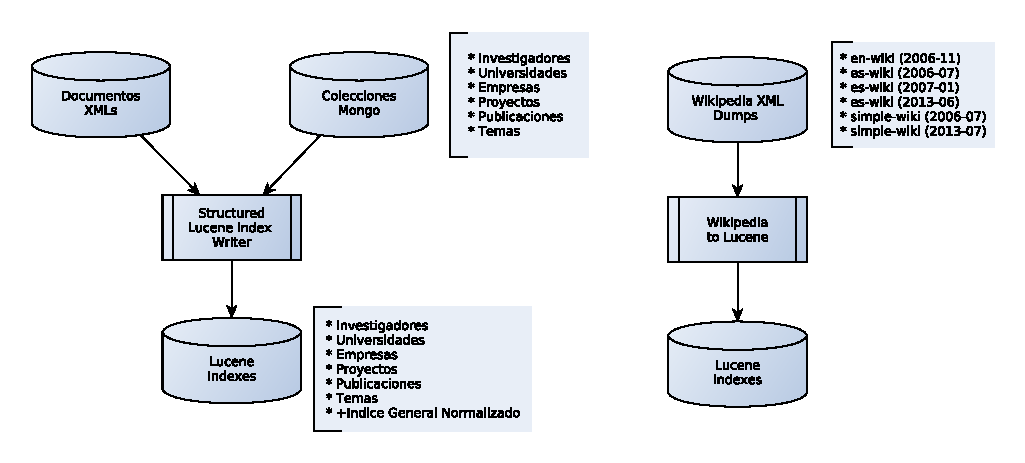
\includegraphics[scale=0.86]{graficos/LuceneWritersJuntos}
  \caption{Creación de Indices}
  \label{fig:LuceneIndexWriterBoth}
\end{figure}

A partir de esta base de datos de mongo y de los archivos xml fueron construidos cinco \'indices
de b\'usqueda lucene y un \'indice de b\'usqueda m\'as, general, con la
informaci\'on normalizada de los otros cinco. 
Cada uno de los cinco índices por entidad mantiene la estructura del tipo como campos de los documentos.
Esto quiere decir que el índice invertido para \emph{Investigadores} tiene los mismos campos
del modelo de datos de nosql. Además, se agregó el campo ``all" que resulta de la concatenación de
todos los campos. Este campo resulta útil a la hora de filtrar resultados. 
El índice general posee un documento por cada entidad de las cinco colecciones, 
manteniendo también un puntero a la entidad original y su tipo.
%El proceso de creación de índices se ilustra en la Figura \ref{fig:LuceneIndexWriterEstructurado}%~\nameref{fig:LuceneIndexWriterEstructurado}.

% \begin{figure}[H]
%   \centering
%     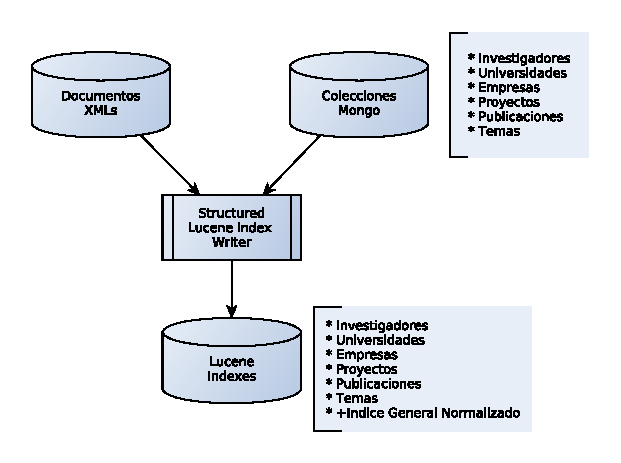
\includegraphics{graficos/LuceneIndexWriterEstructurado}
%   \caption{Lucene Index Writer para datos del proyecto Mitic}
%   \label{fig:LuceneIndexWriterEstructurado}
% \end{figure}

Para la construcción de indices lucene con los dumps de wikipedia usamos la librería gwtwiki (Ver Apéndice~\ref{sec:gwtwiki}).
Los artículos se indexan como documentos con los siguiente campos: \emph{id, title, body y all}. En este proceso se descartan artículos mal formados y 
entradas representado imágenes o discusiones, tal como se sugiere en la guía. 
Por mera curiosidad, tomamos tiempos en la contrucción de estos índices locales sobre versiones de wikipedia.
Estos son algunos tiempos de indexación para distintos dumps sobre una [[detalles de la compu]]:
\begin{center}
\begin{tabular}{| l | l | l | l |}
\hline
Idioma & Tamaño & \# Entradas & Tiempo \\ \hline
es & 50M & \# 16 millones & 2.5min \\ \hline
es & 50M & \# 16 millones & 2.5min \\ \hline
es & 50M & \# 16 millones & 2.5min \\ \hline
es & 50M & \# 16 millones & 2.5min \\ \hline
\end{tabular}
\end{center}

El proceso de creación de índices está ilustrado en la figura \ref{fig:LuceneIndexWriterBoth}



% \begin{figure}[H]
%   \centering
%     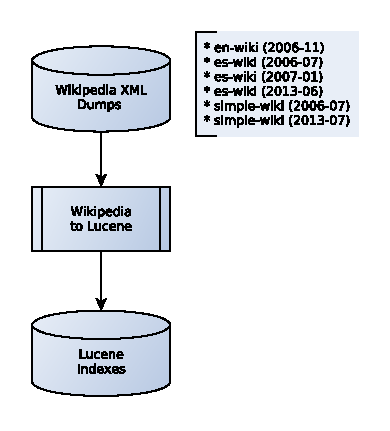
\includegraphics{graficos/LuceneIndexWriterWiki}
%   \caption{Lucene Index Writer para dumps de Wikipedia}
%   \label{fig:LuceneIndexWriterWiki}
% \end{figure}



\subsection{Interfaz de servicios}

La creación offline de índices lucene tiene como finalidad optimizar
la base de conocimiento para responder con mayor eficiencia 
a búsquedas de resultados en un momento posterior. 
En esta sección vamos a ver la interfaz que presenta la base de conocimientos indexada 
al resto de los módulos del sistema y qué dependencias existen con los módulos de
análisis lingüístico.

Para la base de conocimiento estructurada, reutilizamos un modelo de datos
escrito en java  del grafo de entidades que obtuvimos de los investigadores del proyecto mitic (Ver \ref{sec:modelos-morphia}).
A estos modelos se les agregó soporte para su representación como documento dentro de un índice.
Por ejemplo, el modelo para la entidad "Universidad de Buenos Aires", un objeto de clase "UniversidadNodo", además de
persistirse en la colección UniversidadesGrafo de la base de datos de mongo también dispone de una representación como documento en 
un índice lucene particular UniversidadesIndex y otra en el índice general (GeneralIndex).
A nivel colecciones, cada entidad dispone de un representante que maneja el acceso a su colección en la base de datos y también a su índice. A partir de estos representantes por entidad que ofrecen acceso a una base de datos y a un índice creamos la interfaz \emph{KnowlegdeBase}. Las responsabilidades de esta interfaz se corresponden como un handler de conocimiento acerca de una cierta clase de entidades. 
En este punto del código reificamos entidades implicitas en el modelo. Estas entidades son, por ejemplo: Ciudad, Provincia, Centro de Investigación, etc.
Entre otras funcionalidades, cada $KnowledgeBase$ dispone de varios motores de generación de queries acordes al tipo de datos del índice.
Otra de sus responsabilidades es verificar por la identidad de una entidad. Es decir, cada KnowledgeBase sabe responde, dado un string, si ese string \textit{es} una entidad o no lo es, con un cierto grado de confianza. 

\bigskip
[[Reificacion de entidades como algo]]
\bigskip
[[Tablita con totales por entidad]]
\bigskip
[[Relaciones solo presentes en mongo]]
\bigskip

Las \emph{KnowledgeBase} de las cinco entidad y el índice general están, a su vez, controlados por la interfaz \emph{KnowlegdeManager} (KM). 
Las principales tareas de las que se hace cargo el KnowledgeManager en el proceso de generación de respuesta son:

\begin{itemize}
\item Verificar si un string se corresponde con una entidad (y de qu\'e tipo)
\item Verificar si un string est\'a relacionado con el valor de alg\'un atributo de alguna
entidades (por ejemplo: si est\'a presente en el campo especialidades de varias empresas)
\item Verificar si un string es un nombre de campo (areas\_inv,carreras, disciplina) o es un nombre de colecci\'on (universidades,empresas).
\item Devolver una lista de documentos rankeados para una query (usando el índice general)
\end{itemize}

\begin{figure}
  \centering
    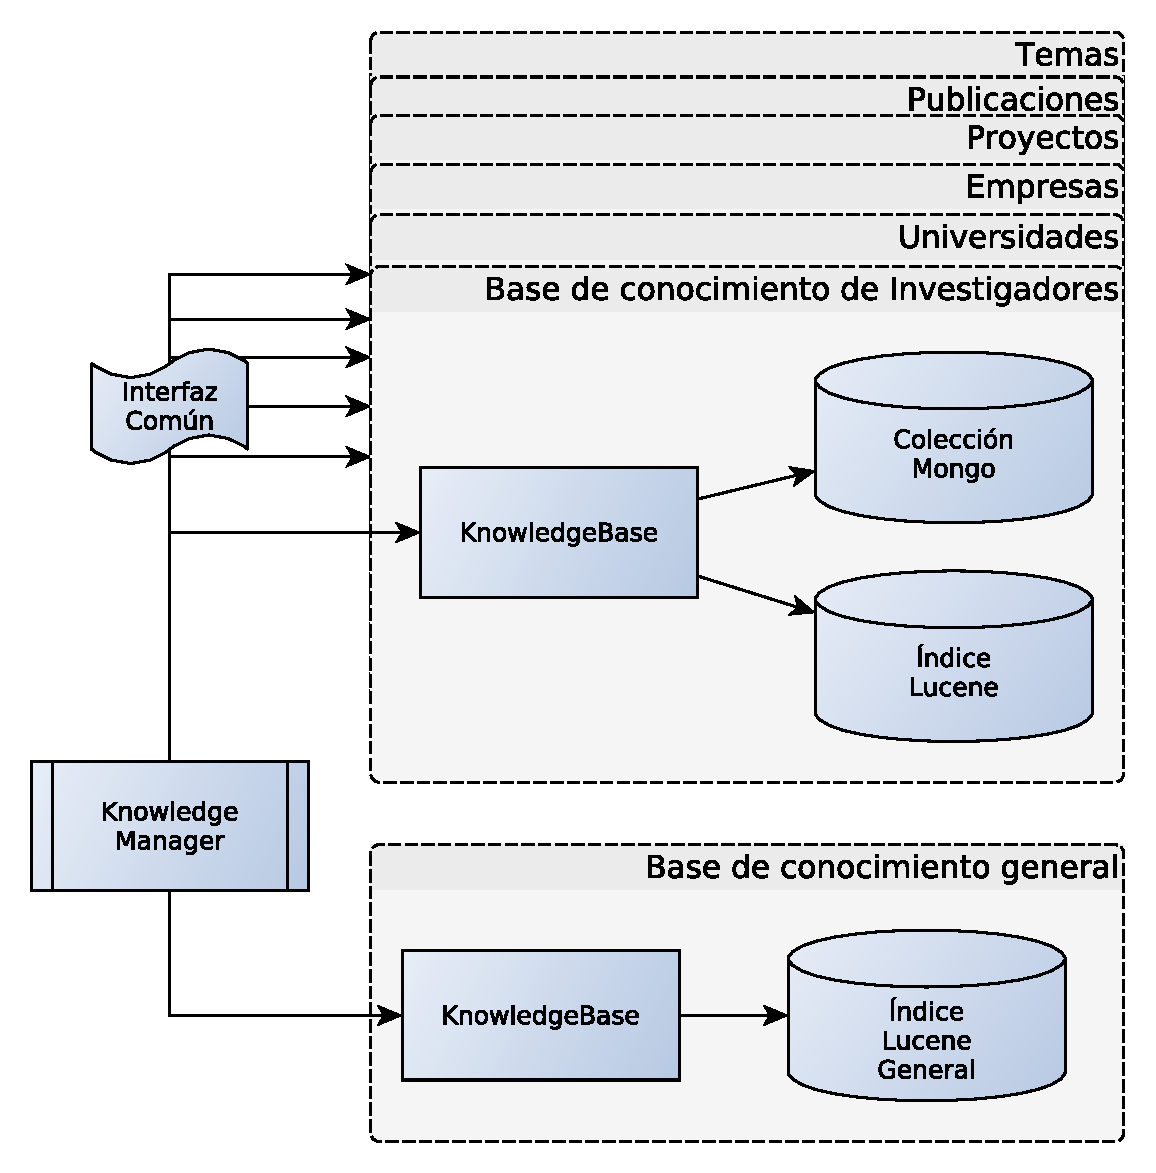
\includegraphics[scale=0.5]{graficos/KnowledgeManager}
  \caption{Base de Conocimiento de grafo de tics}
  \label{fig:KnowledgeManager}
\end{figure}

La base de conocimiento de los ejercicios de wikipedia es mucho más sencilla 
porque no existe ningún modelo \emph{a priori} más allá del documento de lucene.
El formato de la entidad ``artículo", como señalamos antes, es: $(id, titulo, cuerpo)$. 
En este caso, el trabajo más fino no está en el modelado inicial del dominio 
sino la capacidad lingüística de extraer pasajes a partir de un artículo y recomponer información
estructurada a partir de estos pasajes. Mientras que para un modelo estructurado la base de conocimiento
debería permitirnos, para un cierto input, identificar univocamente una entidad y darnos pistas sobre un pedido de
información acerca de esa entidad, el objetivo sobre un corpus de documentos en 
traer todos los documentos en los que sea posible que exista un pasaje respondiendo a la pregunta o
evidencia relevante para apoyar una respuesta. Es decir, mientras una respuesta acotada es una virtud para
el manejador de una base de conocimientos estructurada, el manejador de una lista de documentos de texto debería devolver
una lista lo suficientemente grande para contener la respuesta dentro de los pasajes. La razón de esta política es que si
por ser demasiado estrictos a la hora de retornar documentos llegasemos a descartar un pasaje candidato válido esto
redundaría en una baja generar de efectividad, mientras que en pasos subsiguiente será trivial descartar toda información irrelevante
sin tanto costo. Por eso, el acceso a los indices de wikpedia consta simplemente de un generador de queries similar al recién comentado
accediendo y acumulando resultados (rankeados) a partir de un $LuceneIndexReader$ común (Ver \ref{sec:lucene} para más información).


\bigskip

\section{An\'alisis de la pregunta}

El segundo paso comienza con la detecci\'on del idioma de la pregunta. A
partir de esta detecci\'on se decide qu\'e m\'odulos se utilizar\'an
para analizar la consulta y generar las anotaciones y descomposiciones
en el resto del an\'alisis.

En esta secci\'on detallaremos el procesamiento realizado sobre la
pregunta


\bigskip

\textbf{QAnalyzer} es la clase que implementa el an\'alisis de la
pregunta.

Este es el\textbf{ algoritmo}:


\begin{enumerate}
\item Detectar idioma de la pregunta: los siguientes pasos priorizar\'an
distintos analizadores de acuerdo al idioma reconocido. 
\item Detectar NERs. 
\item Detectar QWords
\item Detectar N-Gramas (1..n)
\item Detectar nombres de campos
\item Detectar nombres de colecciones
\item Detectar verbos
\item Eliminar palabras triviales
\end{enumerate}

Los pasos 1 y 4 consisten en corroborar contra el KnowledgeManager los
NERs que devuelven los analizadores y las distintos N-Gramas de 1 a n
(actualmente n = 4). 


\bigskip

Los pasos 5 y el 6 simplemente verifican igualdad en los sets de tokens
({\textquotedblleft}universidades{\textquotedblright},
empresas{\textquotedblright}, etc)


\bigskip

Si en el paso 8 se procesaron menos del 80\% de los tokens de la
palabra, el sistema se da 

por vencido y devuelve una lista de score docs.

Si no, realiza un an\'alisis estructurado bas\'andose en la
informaci\'on obtenida.


\bigskip

\subsection{M\'odulo de Detecci\'on de idiomas}

Evaluamos distintas herramientas de detecci\'on de idiomas. Enumerar.
Comentar cosas de otras herramientas. En general, los resultados son
muy buenos. Casos borde donde pueden fallar o no, o donde el resultado
no es obvio: {\textquotedblleft}where is the universidad de buenos
aires{\textquotedblright}. Este problema est\'a particularmente
presente en el procesamiento de preguntas, dado que son textos cortos
en los que una construcci\'on sustantivada en otro idioma puede
desequilibrar err\'oneamente la balanza. 

El m\'odulo de detecci\'on de idiomas de nuestro sistema utiliza dos
algoritmo de detecci\'on 

distintos, uno de la biblioteca Freeling y otro de Cybozu Labs, ambos
escritos en java. 

El detector de Cybozu est\'a construido sobre modelos extra\'idos de las
distintas wikipedias y posee una eficacia del 99\% para 49 idiomas,
seg\'un presentaci\'on. Ciertamente, es un muy buen detector de
idiomas. El detector \ de idiomas de freeling es as\'i y as\'a.

Ambos permiten priorizar la detecci\'on de ciertos idiomas sobre otros.
De esta manera podemos forzarlos a identificar s\'olo los idiomas
esperados en nuestro dominio. 

En nuestro sistema, configuramos ambos detectores para emitir un
veredicto s\'olo en caso de confianza alta. El detector obtiene los
resultados de ambos y desempata con un algoritmo ad-hoc en caso de
resultados contradictorios.

\subsection{M\'odulo de Traducci\'on}

Por el momento, no estamos utilizando ning\'un m\'odulo de traducciones:
todo el enfoque multiling\"ue est\'a dado por la detecci\'on del idioma
de la pregunta y la determinaci\'on de distintas herramientas de
an\'alisis seg\'un qu\'e idioma sea. Sin embargo, en un momento se
evalu\'o un enfoque distinto, basado en la traducci\'on. Por ejemplo:
utilizar m\'odulos de procesamiento s\'olo en ingl\'es y
{\textquotedblleft}normalizar{\textquotedblright} los inputs en otros
idiomas (en principio, en espa\~nol), a este idioma interno, y luego lo
mismo con la generaci\'on de respuestas. A pesar de que no es el
enfoque actual, hubo una fase de investigaci\'on dentro del dominio de
la traducci\'on, que result\'o en un m\'odulo de traducci\'on basado en
MyMemoryAPI.

Intento con google translator y la privatizaci\'on. ?`La falta de
software de traducci\'on offline? El m\'odulo de mymemory, robado de
alg\'un lugar. El sistema de cobro. 

\subsection{Comparadores}

Dada la frecuencia en la que resultaba necesario comparar dos string,
decidimos reificar la operaci\'on de comparaci\'on como una familia de
clases que implementan Comparadores. 

Gracias a esto se hace posible cambiar las nociones de igualdad o
similaridad en un m\'odulo completo del sistema o en alguna clase
simplemente configurando otro comparador como par\'ametro. \ La
interfaz permite a los distintos comparadores tomar valores binarios
as\'i como tambi\'en valores entre 0 y 1. A su vez, esta considerada la
posibilidad de configurar un umbral (threshold) a partir del cual
redondear un valor entre 0 y 1 a un valor binario. Otro factor que tuvo
mucha utilidad fue la capacidad de anidar comparadores. A nivel
superclase tambi\'en est\'a permitida la posiblidad de ignorar o no
ignorar la diferencia de may\'usculas, aunque este funcionamiento puede
granularizarse en las instancias particulares. Los comparadores sirven,
en general, para comparar tanto strings representando palabras como
string representado listas de palabras (oraciones o textos). Algunos,
en particular, s\'olo sirven para este segundo caso. Los comparadores
disponibles actualmente son los siguientes, en un pseudo-orden
decreciente de exactitud:


\begin{itemize}
\item Equal: compara por igualdad estricta
\item EqualNoPunct: compara por igualdad, eliminando signos de
puntuaci\'on y normalizando acentos y otras posibles diferencias que no
deber\'ian tenerse en cuenta.
\item Contains: verifica si un string contiene a otro
\item EditDistance: no implementado
\end{itemize}
Los siguiente comparadores son algoritmos fueron adaptados a partir de
los Scorers del \ proyecto Qanus. Todos devuelven valores reales entre
0 y 1 y sirven para comparar textos (y no palabras). Estos
comparadores, al igual que Contains, no son sim\'etricos. Para
distinguir, llamaremos primer string al buscado y segundo string a
aquel en el cual se busca el primero. 


\begin{itemize}
\item Frequency: cuenta la cantidad de veces que los tokens del primer
string ocurren en el segundo string. Esta suma se divide por la
longitud del segundo string, dando un valor entre 0 y 1.
\item Coverage: cuenta cuantos tokens del primer string aparecen al
menos una vez en el segundo, y divide esta suma por el total de tokens
del \textit{primer} string.
\item Proximity: computa la distancia de 
\end{itemize}
This feature computes the distance between the occurences of two search
strings within a passage.

Typically the search string may span multiple word tokens in the
passage. 

To compute the distance, we will compute the midpoint of the span of the
two

search strings, and find the difference between the two midpoints. 

\ * \ ... X .. X... X .... Y ... Y

\ * \ \ \ \ \ \ \ \ \ \ {\textbar} \ \ \ \ \ \ \ \ \ \ \ \ \ {\textbar}

\ *
\ \ \ \ \ \ \ \ \ \ \ {\textless}-{}-{}-{}-{}-{}-{}-{}-{}-{}-{}-{}-{\textgreater}

\ * \ where X are matches to search string 1 and Y are matches to the
other search string.


\begin{itemize}
\item TermSpan
\end{itemize}
\ * This feature makes use of the span of matching search terms within a
passage.

\ * For example, suppose the passage has the following search term
matches (denoted by X)

\ * ..... X ..... X ..... X ......

\ * ......a ..... b ...... c .....

\ * 

\ * a, b, c are position of the matching term within the passage (in
terms of words).

\ * The span is thus {\textbar}c-a{\textbar}.

\ * 

\ * The score of this feature is given as 

\ * \ \ \# matching terms / span

\ * 

\ * This score is guaranteed to be between 0 and 1 inclusive.


\bigskip

\textbf{5.2.4.4 M\'odulos de procesamiento de lenguaje natural}

Para el an\'alisis ling\"u\'istico de la pregunta se utilizan distintas
librer\'ias disponibles, dependiendo del idioma detectado. Para idioma
espa\~nol, utilizamos la librer\'ia Freeling, que fue comentada
anteriormente. De esta librer\'ia utilizamos el POS-tagger, el NER y el
NEC (reconocimiento y clasificaci\'on de entidades nombradas,
respectivamente). Para el ingl\'es, utilizamos en parte los m\'odulos
de Freeling y en parte herramientas producidas por la universidad de
Stanford, tomados de Qa-sys. El motivo por el que usamos dos
librer\'ias distintas es el esperado: los m\'odulos de Stanford
demostraron funcionar mucho mejor que los de Freeling para el ingl\'es.

\subsection{Tecnolog\'ias utilizadas}


\bigskip

\textbf{Stanford Question Classifier }


Stanford POS\newline
Stanford NER

\textbf{Freeling POS}

\textbf{Freeling NER}

QWords, 

Verbos

Trabajo futuro: ?`Otros idiomas?


\bigskip

\section{Generaci\'on de Respuestas}

Una vez completada la generaci\'on de
metadatos ling\"u\'isticos, se procede al tercer paso, que toma
diferentes formas dependiendo de la informaci\'on encontrada en el
an\'alisis de la pregunta.


Dependiendo de cu\'anto se haya procesado de la pregunta original,
existen dos tipos de flujos distintos de generaci\'on de respuestas: el
estructurado y el no estructurado.

La generaci\'on de respuestas estructurada se construye cuando la
informaci\'on obtenida en el an\'alisis ling\"u\'istico es suficiente
para generar un mapeo coherente a la ontolog\'ia definida
impl\'icitamente por la base de conocimientos. El an\'alisis no
estructurado se ejecuta cuando la informaci\'on generada no fue
suficiente y consiste en intentar ubicar marcas que puedan reconducir
al an\'alisis al flujo estructurado (es decir, se intentan diferentes
transformaciones a fin de identificar informaci\'on que permita el
an\'alisis estructurado). Esto se realiza con m\'etodos menos
confiables y menos r\'apidos que en el an\'alisis ling\"u\'istico
inicial. Si el an\'alisis falla en esta segunda barrera, se procede a
dar una respuesta ad-hoc con la informaci\'on disponible. 

En flujo de respuesta estructurado depende de la cantidad de
informaci\'on que se haya identificado. Esta informaci\'on, en este
punto, tiene tres tipos: QType, NERs y verbos. 




\begin{figure}
  \centering
    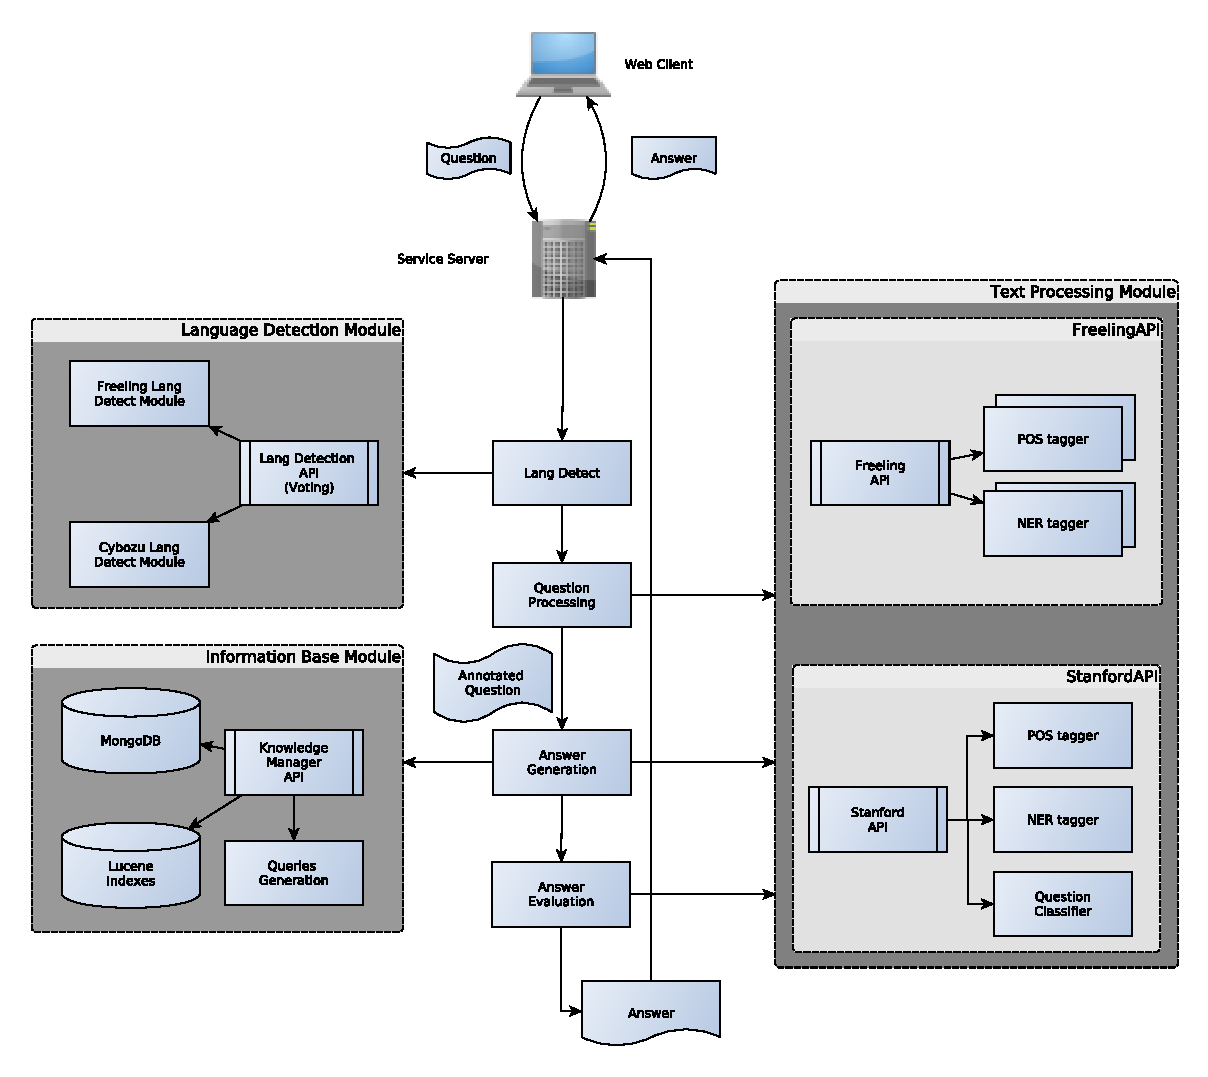
\includegraphics[scale=0.86]{graficos/Architecture}
  \caption{Arquitectura}
  \label{fig:Architecture}
\end{figure}

Como dice en \cite{greenwade93} y también en \cite{RE1}
%\end{document}
